% This file was created with tikzplotlib v0.9.12.
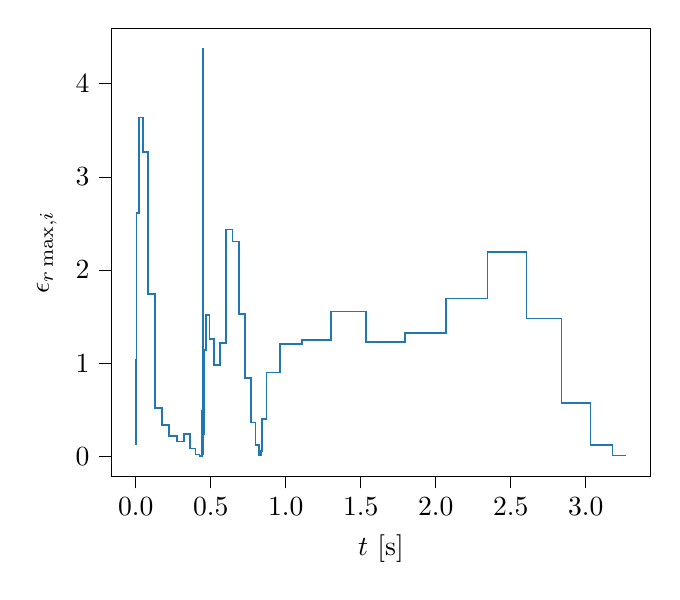
\begin{tikzpicture}

\definecolor{color0}{rgb}{0.12156862745098,0.466666666666667,0.705882352941177}

\begin{axis}[
tick align=outside,
tick pos=left,
x grid style={white!69.0196078431373!black},
xlabel={\(\displaystyle t\) [s]},
xmin=-0.163529513089662, xmax=3.4341197748829,
xtick style={color=black},
xtick={-0.5,0,0.5,1,1.5,2,2.5,3,3.5},
xticklabels={
  \(\displaystyle {\ensuremath{-}0.5}\),
  \(\displaystyle {0.0}\),
  \(\displaystyle {0.5}\),
  \(\displaystyle {1.0}\),
  \(\displaystyle {1.5}\),
  \(\displaystyle {2.0}\),
  \(\displaystyle {2.5}\),
  \(\displaystyle {3.0}\),
  \(\displaystyle {3.5}\)
},
y grid style={white!69.0196078431373!black},
ylabel={\(\displaystyle \epsilon_{r\max,i}\)},
ymin=-0.216228659419286, ymax=4.59531445943358,
ytick style={color=black},
ytick={-1,0,1,2,3,4,5},
yticklabels={
  \(\displaystyle {\ensuremath{-}1}\),
  \(\displaystyle {0}\),
  \(\displaystyle {1}\),
  \(\displaystyle {2}\),
  \(\displaystyle {3}\),
  \(\displaystyle {4}\),
  \(\displaystyle {5}\)
}
]
\addplot [semithick, color0, const plot mark right]
table {%
0 0.121983402984149
0.0056120056173798 1.0397347237579
0.0221666130741685 2.60893420999731
0.0488337052264625 3.63845013596332
0.0842760827216659 3.26490555518246
0.12671651675769 1.74163021403044
0.174026866756148 0.516152625860825
0.223834794217301 0.33450836270812
0.273642721678455 0.220384136726914
0.320953071676913 0.160813135877187
0.363393505712937 0.242209298496741
0.39883588320814 0.0863267735993829
0.425502975360434 0.0214895788321281
0.442057582817223 0.00247784598311719
0.447669588434603 0.484419099974106
0.447669588434603 0.484419099974106
0.447694744492815 1.05729575546193
0.447768951264519 4.37660795403118
0.447888487688025 1.39055441719649
0.448047359718729 1.08701511130451
0.448237600848921 1.00897329734691
0.448449671593784 0.819735968241424
0.448672937840577 0.883128142621403
0.44889620408737 0.879965656487038
0.449108274832234 0.612952202451126
0.449298515962425 0.593879976766317
0.44945738799313 0.382865802989038
0.449576924416636 0.396351874180598
0.44965113118834 0.0262547409479423
0.449676287246552 0.0234699890399677
0.449676287246552 0.0234699890399677
0.454574962603674 0.241927617611714
0.469025348637549 1.14270435371074
0.492302842652881 1.51552999136163
0.523240213901389 1.26238085731676
0.560286133405463 0.983098163887864
0.60158296407088 1.21610552287315
0.645059910367528 2.43550501989112
0.688536856664177 2.30561833770312
0.729833687329594 1.52511995353691
0.766879606833668 0.842768120129724
0.797816978082176 0.365550642291069
0.821094472097507 0.125859418996696
0.835544858131383 0.0143620116495248
0.840443533488505 0.0583681437583286
0.840443533488505 0.0583681437583286
0.87129471129975 0.40283487740658
0.962301237854726 0.901074100358903
1.10889966590181 1.20885923751466
1.30373893811699 1.24705321152683
1.53704899981345 1.55701767541929
1.79713071027977 1.2276836460883
2.0709424865465 1.32473440536887
2.34475426281323 1.69475109679354
2.60483597327954 2.19468347947709
2.838146034976 1.47995313043799
3.03298530719118 0.574563811500261
3.17958373523827 0.119461624485707
3.27059026179324 0.00896155986365053
};
\end{axis}

\end{tikzpicture}
